\chapter{rotary club}
\label{sec:rotaryclub}
\lstset{style=68KStyle}
\lhead[tempest 2000]{}

Sprinkled throughout \icode{yak.s}, the principal source code file for \textit{Tempest 2000}, we
find references to a never-produced 'rotary controller'. This was a device that would emulate
the controller present in the coin-operated original of Tempest in 1981.

Towards the end of the \icode{Frame} interrupt routine we find the main logic used to detect
and, if a rotary controller is present, detect its input:
\begin{lstlisting}
        ; Check for joypad input. The logic for rotary controllers
        ; was added to support the potential release of a rotary
        ; controller for the Jaguar, but this never happened.
        ; So all rotary controller logic in Tempest 2000 is unused.
        tst roconon           ; Is Rotary Controller enabled?
        bne roco              ; Yes, do the rotary controller.
        jsr dopad             ; No, check for normal joypad input.
        bra exxit             ; We're done - so exit interrupt.
    
        ; Logic for reading input from the never-built and never-
        ; released rotary controller. We only look for button input
        ; every 8 interrupts.
roco:   move pitcount,d1      ; Get the rotary input interval counter.
        and #$07,d1           ; Do a modulus 7 on the counter.
        bne rotonly           ; If non-zero, read the rotary control only.
        jsr dopad             ; Otherwise, look for button presses too.
rotonly:
        add #1,pitcount       ; Increment the interval counter.
        bsr readrotary        ; Read input from the rotary controller.
\end{lstlisting}
You might wonder how it was possible to test a rotary controller that doesn't exist.
The answer to this is that you make one of your own. In this case, Yak adapted a 
an Atari drive controller marketed for the antiquated Atari 2600 game console and used
it as a substitute for the rotary input promised by the Jaguar hardware team.

\begin{figure}[H]
    \centering
    \begin{adjustbox}{width=4cm,center}
      \frame{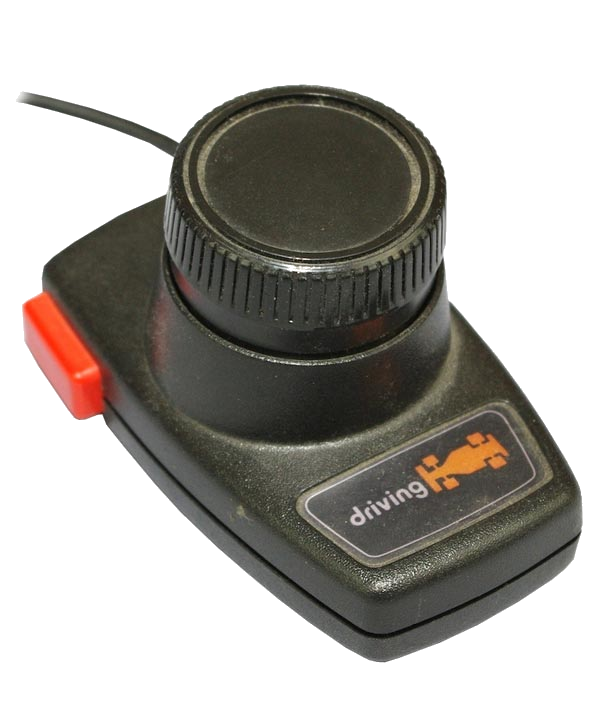
\includegraphics[width=12cm]{src/rotary/rotary.png}}%
    \end{adjustbox}
\caption*{The humble 2600 Atari drive controller.}
\end{figure}

Once we've decided we're reading from this hacked-up rotary controller our first task is to hide it
behind some secret button presses on the options screen.

\begin{lstlisting}
selector:
        cmp.l #option2,the_option ; Are we on the 'Options' screen?
        bne selector2             ; If not, skip.
        btst.b #6,sysflags        ; Are controllers enabled?
        bne sopt2                 ; If not, skip.
        btst.b #4,pad_now         ; Pause pressed by Player 1?
        beq selector2             ; If not, skip.
        btst.b #4,pad_now+4       ; Pause pressed by Player 2?
        beq selector2             ; If not, skip.
        bset.b #6,sysflags        ; Enable controllers.
        jsr sayex                 ; Say 'Excellent!'.
\end{lstlisting}
If we have 2 controllers and both press the pause button it enables us to select the controller
type and enable the rotary controller:
\begin{figure}[H]
    \centering
    \begin{adjustbox}{width=10cm,center}
      \frame{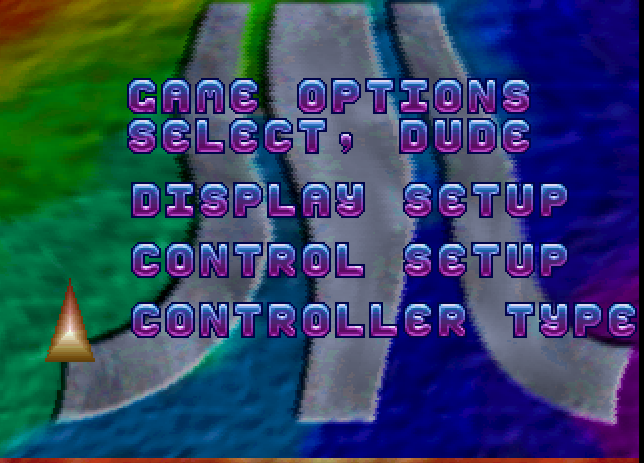
\includegraphics[width=4cm]{src/rotary/controller_type.png}}%
      \hspace{0.5cm}
      \frame{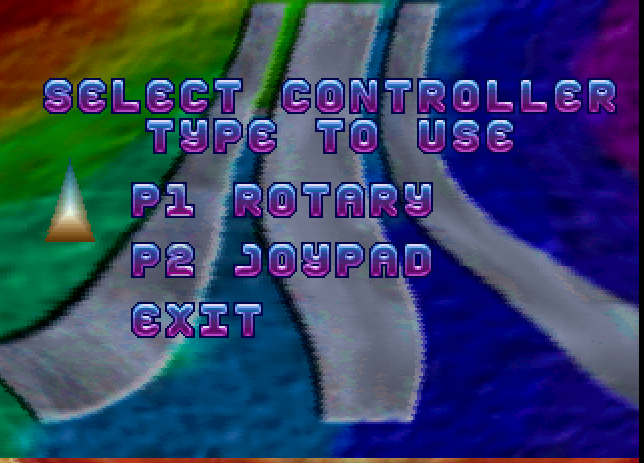
\includegraphics[width=4cm]{src/rotary/rotary_select.png}}%
    \end{adjustbox}
  \caption*{Selecting and enabling the rotary controller.}
\end{figure}

Next we have to figure out what it's telling us. For this, and for the ordinary joypad controller too,
we inspect a 4-byte phrase (\icode{JOYIN}) that tells us what buttons or dials have been pressed most recently.
These 4 bytes are a bitmap: if a bit is set it tells us a specific button has been pressed. 

\begin{figure}[H]
  {
    \setlength{\tabcolsep}{3.0pt}
    \setlength\cmidrulewidth{\heavyrulewidth} % Make cmidrule = 
    \begin{adjustbox}{width=8cm,center}

      \begin{tabular}{lll}
        \toprule
        Button & Hex & Bitmap\\
        \midrule
       \icode{abutton }     & \icode{20000000} & \icode{00100000000000000000000000000000} \\
       \icode{pausebutton } & \icode{10000000} & \icode{00010000000000000000000000000000} \\
       \icode{bbutton }     & \icode{02000000} & \icode{00000010000000000000000000000000} \\
       \icode{right }       & \icode{00800000} & \icode{00000000100000000000000000000000} \\
       \icode{left }        & \icode{00400000} & \icode{00000000010000000000000000000000} \\
       \icode{down }        & \icode{00200000} & \icode{00000000001000000000000000000000} \\
       \icode{up }          & \icode{00100000} & \icode{00000000000100000000000000000000} \\
       \icode{seven }       & \icode{00080000} & \icode{00000000000010000000000000000000} \\
       \icode{four }        & \icode{00040000} & \icode{00000000000001000000000000000000} \\
       \icode{one }         & \icode{00020000} & \icode{00000000000000100000000000000000} \\
       \icode{asterisk }    & \icode{00010000} & \icode{00000000000000010000000000000000} \\
       \icode{cbutton }     & \icode{00002000} & \icode{00000000000000000010000000000000} \\
       \icode{optionbutton }& \icode{00000200} & \icode{00000000000000000000001000000000} \\
       \icode{two }         & \icode{00000080} & \icode{00000000000000000000000010000000} \\
       \icode{five }        & \icode{00000040} & \icode{00000000000000000000000001000000} \\
       \icode{eight }       & \icode{00000020} & \icode{00000000000000000000000000100000} \\
       \icode{zerobutton }  & \icode{00000010} & \icode{00000000000000000000000000010000} \\
       \icode{three }       & \icode{00000008} & \icode{00000000000000000000000000001000} \\
       \icode{six }         & \icode{00000004} & \icode{00000000000000000000000000000100} \\
       \icode{nine}        & \icode{00000002} & \icode{00000000000000000000000000000010} \\
       \icode{hash}        & \icode{00000001} & \icode{00000000000000000000000000000001} \\
        \bottomrule
      \end{tabular}
    \end{adjustbox}
  }\caption*{All controller buttons and the bit they set in the \icode{JOYIN} bitmap.}
\end{figure}

\icode{readrotary} does this job. It is only interested in a subset of the buttons. These are:

\begin{figure}[H]
  {
    \setlength{\tabcolsep}{3.0pt}
    \setlength\cmidrulewidth{\heavyrulewidth} % Make cmidrule = 
    \begin{adjustbox}{width=8cm,center}

      \begin{tabular}{lll}
        \toprule
        Button & Hex & Bitmap\\
        \midrule
       \icode{right }       & \icode{00800000} & \icode{00000000100000000000000000000000} \\
       \icode{left }        & \icode{00400000} & \icode{00000000010000000000000000000000} \\
        \bottomrule
      \end{tabular}
    \end{adjustbox}
  }
\end{figure}

But the rotary controller has everything in a slightly different position, so when we read \icode{JOYIN},
we'll find the right and left movement bits 4 bits to the left like so:

\begin{figure}[H]
  {
    \setlength{\tabcolsep}{3.0pt}
    \setlength\cmidrulewidth{\heavyrulewidth} % Make cmidrule = 
    \begin{adjustbox}{width=8cm,center}

      \begin{tabular}{lll}
        \toprule
        Button & Hex & Bitmap\\
        \midrule
       \icode{right }       & \icode{08000000} & \icode{00001000000000000000000000000000} \\
       \icode{left }        & \icode{04000000} & \icode{00000100000000000000000000000000} \\
        \bottomrule
      \end{tabular}
    \end{adjustbox}
  }
\end{figure}

Thus \icode{readrotary}'s first task is to extract the most recently pressed buttons and get them
into the register \icode{d0}. It must then move everything 4 bits to the right. It does this as follows.
\begin{lstlisting}
readrotary:
    btst.b #3,sysflags     ; Rotary controller enabled for Player 1?
    beq op2                ; If not, skip to checking Player 2.
    move.l   #$f0fffffc,d1 ; d1 = Joypad data mask   (Player 1)
    moveq.l  #$ffffffff,d2 ; d2 = Cumulative joypad reading
    move.w   #$81fe,JOYOUT ; Ask for the most recent button presses.
    move.l   JOYIN,d0      ; Read joypad, pause button, A button
    or.l     d1,d0         ; Mask off unused bits
    ; Rotate d0 4 bits to the right so that the bits are where we
    ; expect them to be.
    ror.l    #4,d0         ; Shift everything 4 bits to the right.
    and.l    d0,d2         ; d2 = xxAPxxxx RLDUxxxx xxxxxxxx xxxxxxxx
    swap     d2            ; Swap position of the first 2 with last 2 bytes.
    move     d2,d0         ; Store result in d0.

    lea lstcon,a1          ; Point a1 at lstcon (last read from controller).
    lea roconsens,a2       ; Point a2 at roconsens.
    bsr rroco              ; Calculate the input movement and store in d0.
    add.l d0,rot_cum       ; Add result to the cumulative movement.
op2:
    ; We omit the duplicated logic for player 2.
    rts
\end{lstlisting}
Once we have a value to work with, the question is how we decide if it's telling us to move the 
claw right or left. What we will do is compare the current input with the last input reported
by the controller and depending on whether it is before or after the input value's position in
the \icode{conseq} array move it right or left, respectively.

\begin{lstlisting}
conseq: dc.b 0,1,3,2
\end{lstlisting}

We can capture some of these potential outcomes as follows. 
\begin{figure}[H]
  {
    \setlength{\tabcolsep}{3.0pt}
    \setlength\cmidrulewidth{\heavyrulewidth} % Make cmidrule = 
    \begin{adjustbox}{width=6cm,center}

      \begin{tabular}{lll}
        \toprule
        Previous Value & Current Value & Result\\
        \midrule
       \icode{1}       & \icode{0} & \icode{Move Right} \\
       \icode{1}       & \icode{3} & \icode{Move Left} \\
       \icode{3}       & \icode{1} & \icode{Move Right} \\
       \icode{3}       & \icode{2} & \icode{Move Left} \\
       \icode{2}       & \icode{3} & \icode{Move Right} \\
       \icode{2}       & \icode{0} & \icode{Move Left} \\
       \icode{0}       & \icode{2} & \icode{Move Right} \\
       \icode{0}       & \icode{1} & \icode{Move Left} \\
        \bottomrule
      \end{tabular}
    \end{adjustbox}
  }
\end{figure}

It's not exactly intuitive why this is the case.

But anyway, here is the code that does the job.
\begin{lstlisting}
rroco:
        rol.b #2,d0         ; Phase Bits to bottom of word
        and #$03,d0         ; Get juicy bits
        move (a1),d4        ; Put last value read (lstcon) in d4.
        cmp d4,d0           ; Compare to most recent read.
        beq decsens         ; Did not move, so exit early.

        move d0,(a1)        ; Store current read in lstcon.
        lea conseq,a0       ; Point to sequence values
        clr d5              ; Set d5 to 0.

        ; Search sequence values (conseq) for a match to the last value
        ; we read (lstcon).
slocate:
        cmp.b 0(a0,d5.w),d4 ; Get val using d5 as index into conseq.
        beq slocated        ; If it equals last value read (d4), exit loop.
        addq #1,d5          ; Otherwise, increment d5..
        bra slocate         ; .. and loop.
    
        ; d5 now points to the position in conseq matching the previous
        ; value read from the rotary controller. To determine whether 
        ; to move left or right we now see if the currently read value
        ; is before (right) or after (left) the most recent value read
        ; from the controller.
slocated:
        subq #1,d5          ; Subtract 1 from d5.
        and #3,d5           ; Clamp to 0 - 7.
        cmp.b 0(a0,d5.w),d0 ; Use it as in index into conseq.
        beq rclaw_right     ; If val is equal to d0(curr read), move right.
        addq #2,d5          ; Add two to d5
        and #3,d5           ; Clamp to 0 - 7.
        cmp.b 0(a0,d5.w),d0 ; Use it as in index into conseq.
        beq rclaw_left      ; If val is equal to d0 (curr read), move left.
        clr.l d0            ; Clear d0.
        rts                 ; Return
\end{lstlisting}
